
\begin{exercise}

% !TEX root = ../main.tex




 De co\"ordinaten van een puntmassa veranderen als volgt:
\begin{eqnarray*}
	x(t)=3t^2\qquad y(t)=2t^4
\end{eqnarray*}
\begin{enumerate}
\item Bepaal de positie van het voorwerp na \SI{2,0}{s}.% en na $4,0\rm\,s$.
\item Bepaal de vergelijking van de baan van het deeltje.
\item Op welk ogenblik bedraagt de grootte van de snelheid \SI{10}{m/s}?
\item Teken de snelheidsvector op de baan op dat ogenblik. Welke hoek maakt ze met de $x$-as?
\end{enumerate}

\begin{oplossing}
\item[(a)] De plaatsvector op $t=\SI{2,0}{s}$ is $\vec{r}=12\,\vec{e}_x+32\,\vec{e}_y$.
\item[(b)] De vergelijking van de baan vinden we door de paramater $t$ te elimineren uit de uitdrukkingen voor $x(t)$ en $y(t)$.
\begin{eqnarray*}
x=3t^2\Leftrightarrow t^2&=&\frac{x}{3}\\
&\Downarrow&\mathrm{substitutie}\\
y&=&2t^4=2\left(\sqrt{\frac{x}{3}}\right)^4=\frac{2}{9}x^2
\end{eqnarray*}
Aangezien $x(t)$ niet negatief kan worden, is de baan een halve parabool.

\item[(c)]De grootte van de snelheid vinden we met stelling van Pythagoras, omdat we immers de componenten van de snelheid kunnen bepalen.
\begin{eqnarray*}
v(t)&=&\sqrt{v_x^2(t)+v_y^2(t)}\\
&=&\sqrt{(6t)^2+\left(8t^3\right)^2}\\
\end{eqnarray*}
Om te weten wanneer die gelijk aan \SI{10}{m/s}, lossen we de volgende vergelijking op naar $t$.
\begin{eqnarray*}
10=\sqrt{(6t)^2+\left(8t^3\right)^2}&\Leftrightarrow&t=\pm 1
\end{eqnarray*}
Als we alleen positieve tijdstippen bekijken, houden we $t=\SI{1}{s}$ over. 
\item[(d)]De snelheidsvector is getekend in de figuur.
\begin{figure}[ht!]
\begin{picture}(390,160)(0,0)
\put(130,0){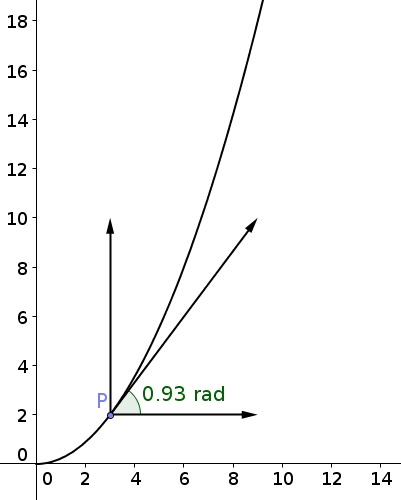
\includegraphics[width=0.3\textwidth]{dyn/exercises/12p53}}
\put(200,30){$\vec{v}_x$}
\put(200,65){$\vec{v}$}
\put(150,70){$\vec{v}_y$}
\put(205,120){$y(x)$}
\end{picture}
\end{figure}
\newline
De hoek vinden we uit $\tan\alpha=\frac{v_y}{v_x}$ als $\alpha=\bgtan\!{\left(\frac{8}{6}\right)}=0,93\rm\,rad=\SI{55,13}{\degree}$.
\end{oplossing}


\end{exercise}
